\documentclass[conference]{IEEEtran}
\IEEEoverridecommandlockouts
\usepackage{cite}
\usepackage{amsmath,amssymb,amsfonts}
\usepackage{algorithmic}
\usepackage{graphicx}
\usepackage{float}
\usepackage{textcomp}
\usepackage{xcolor}
\usepackage{tabularx}
\usepackage{newtxtext}
\usepackage{multirow}
\usepackage{booktabs}
\def\BibTeX{{\rm B\kern-.05em{\sc i\kern-.025em b}\kern-.08em
    T\kern-.1667em\lower.7ex\hbox{E}\kern-.125emX}}
\usepackage{tikz}

\usetikzlibrary{
    positioning,
    fit,
    arrows.meta
}
\begin{document}


\title{Perbandingan Metode Rule-Based dan Decision Tree C4.5 untuk Penentuan Prioritas Pengiriman Invoice}

\author{\IEEEauthorblockN{1\textsuperscript{st} First Author}
% \IEEEauthorblockA{\textit{Institution} \\
% City, Country \\
% email@institution.ac.id}
\and
\IEEEauthorblockN{2\textsuperscript{nd} Second Author}
% \IEEEauthorblockA{\textit{Institution} \\
% City, Country \\
% email@institution.ac.id}
}

\maketitle

% --- PEMANGGILAN KOMPONEN DOKUMEN ---
\begin{abstract}
Pengiriman \textit{invoice} merupakan proses administrasi penting karena berhubungan langsung dengan penagihan, verifikasi dokumen, dan penerimaan pembayaran. Pada objek penelitian, pelacakan \textit{invoice} dan bukti penerimaan masih dilakukan secara semi-manual sehingga status pengiriman sulit dipantau secara terintegrasi. Selain itu, penentuan prioritas pengiriman masih bergantung pada pengalaman staf administrasi dalam menafsirkan aturan pelanggan, seperti kebijakan \textit{cut-off}, jadwal penerimaan, dan hari penerimaan dokumen. Penelitian ini mengembangkan sistem pelacakan \textit{invoice} dan \textit{Proof of Delivery} (POD) berbasis web dengan membandingkan pendekatan \textit{Rule-Based} dan \textit{Decision Tree} C4.5 untuk menentukan prioritas pengiriman \textit{invoice}. Pengetahuan operasional diperoleh dari regulasi pelanggan, data historis \textit{invoice}, dan diskusi dengan staf administrasi, kemudian diformalkan menjadi atribut, aturan keputusan, dan pedoman pelabelan pakar. Hasil penelitian diharapkan menghasilkan sistem yang mampu mendokumentasikan status pengiriman, menyimpan POD, serta memberikan dasar keputusan prioritas yang lebih konsisten dan dapat dievaluasi.
\end{abstract}

\begin{IEEEkeywords}
\textit{invoice tracking}, \textit{Proof of Delivery}, \textit{Rule-Based}, \textit{Decision Tree} C4.5, prioritas pengiriman
\end{IEEEkeywords}

\section{Pendahuluan}

Invoice merupakan dokumen penting dalam proses administrasi penjualan karena berfungsi sebagai dasar penagihan, pencatatan transaksi, dan proses pembayaran pelanggan. Ketepatan pengiriman invoice memengaruhi kelancaran arus kas perusahaan, terutama bagi pelanggan yang menerapkan aturan administrasi tertentu, seperti batas \textit{cut-off}, jadwal penerimaan dokumen, dan prosedur verifikasi sebelum pembayaran dapat diproses. Oleh karena itu, perusahaan membutuhkan sistem yang tidak hanya mampu melacak status pengiriman invoice, tetapi juga memastikan setiap invoice dikirim sesuai dengan ketentuan operasional pelanggan.

Pada perusahaan yang menjadi objek penelitian, proses pelacakan invoice masih dilakukan secara semi-manual menggunakan \textit{spreadsheet}. Staf administrasi harus memeriksa status pengiriman secara manual serta menentukan prioritas pengiriman berdasarkan pengalaman kerja. Kondisi tersebut menyebabkan proses pencarian status invoice menjadi kurang efisien, keputusan prioritas berpotensi berbeda antarstaf, dan pengetahuan operasional sulit ditransfer kepada staf baru. Selain itu, bukti penerimaan (\textit{Proof of Delivery}/POD) belum terdokumentasi secara terintegrasi sehingga proses penelusuran riwayat pengiriman masih membutuhkan waktu yang relatif lama.

Permasalahan tersebut tidak hanya berkaitan dengan pelacakan dokumen, tetapi juga dengan proses pengambilan keputusan. Prioritas pengiriman invoice dipengaruhi oleh berbagai aturan operasional pelanggan, seperti jenis \textit{cut-off}, jadwal penerimaan dokumen, serta ketentuan administrasi lainnya. Sebagian besar pertimbangan tersebut masih tersimpan sebagai \textit{tacit knowledge} yang dimiliki oleh staf administrasi sehingga belum direpresentasikan secara sistematis ke dalam sistem informasi. Akibatnya, proses penentuan prioritas sangat bergantung pada pengalaman individu dan sulit dievaluasi secara konsisten.

Berbagai penelitian telah mengembangkan sistem \textit{document tracking}, \textit{Proof of Delivery} (POD), maupun model klasifikasi berbasis \textit{Decision Tree} pada berbagai domain operasional \cite{10.1007/978-3-642-55032-4_33,gemma,gunadhya_rajawali_logistik_2021,Siahaan_Doni_2025,firmansyah,afifahdedi}. Meskipun demikian, sebagian besar penelitian masih berfokus pada pelacakan status dokumen atau pembangunan model klasifikasi secara terpisah. Penelitian yang mengkaji proses transformasi pengetahuan operasional menjadi dasar pembentukan model keputusan, serta membandingkan pendekatan \textit{knowledge-driven} dan \textit{data-driven} dalam konteks pengelolaan invoice, masih relatif terbatas.

Berdasarkan permasalahan tersebut, penelitian ini mengusulkan sistem pelacakan invoice dan \textit{Proof of Delivery} (POD) berbasis web yang mengintegrasikan proses \textit{Knowledge Acquisition} dan \textit{Knowledge Formalization} untuk merepresentasikan pengetahuan operasional perusahaan. Pengetahuan tersebut kemudian digunakan sebagai dasar penyusunan pedoman \textit{expert labeling} sehingga diperoleh \textit{ground truth} yang digunakan dalam pembangunan dan evaluasi model. Penelitian ini membandingkan dua pendekatan yang berbeda, yaitu model \textit{Rule-Based} sebagai representasi pengetahuan pakar dan algoritma Decision Tree C4.5 sebagai pendekatan berbasis data.

Kontribusi utama penelitian ini meliputi tiga aspek. Pertama, pengembangan sistem pelacakan invoice dan \textit{Proof of Delivery} (POD) berbasis web yang mendukung pencatatan status dan riwayat pengiriman invoice. Kedua, formalisasi pengetahuan operasional menjadi aturan eksplisit yang digunakan sebagai dasar proses \textit{expert labeling}. Ketiga, evaluasi komparatif antara pendekatan \textit{Rule-Based} dan Decision Tree C4.5 untuk mengetahui kemampuan kedua pendekatan dalam merepresentasikan proses pengambilan keputusan pada penentuan prioritas pengiriman invoice.


```latex
\section{Penelitian Terdahulu}

Tabel \ref{tab:related_work} membandingkan penelitian-penelitian terdahulu yang relevan dengan penelitian ini. Perbandingan dilakukan berdasarkan fokus penelitian, metode yang digunakan, serta keterbatasan masing-masing penelitian. Berdasarkan hasil kajian literatur, sebagian besar penelitian hanya berfokus pada satu aspek, seperti sistem pelacakan dokumen, \textit{Proof of Delivery} (POD), atau implementasi algoritma klasifikasi. Belum ditemukan penelitian yang mengintegrasikan pelacakan invoice, formalisasi pengetahuan operasional, \textit{expert labeling}, serta evaluasi komparatif antara pendekatan Rule-Based dan Decision Tree C4.5 dalam satu kerangka penelitian.

\begin{table}[htbp] \caption{Comparison of Previous Studies} \label{tab:related_work} \centering \renewcommand{\arraystretch}{1.15} \resizebox{\columnwidth}{!}{ \begin{tabular}{lcccc} \hline \textbf{Study} & \textbf{Track} & \textbf{POD} & \textbf{RB} & \textbf{DT} \\ \hline Sunindyo (2014) & \checkmark & -- & -- & -- \\ Acedo (2025) & \checkmark & \checkmark & -- & -- \\ Gunadhya (2021) & -- & \checkmark & -- & -- \\ Firmansyah (2021) & -- & -- & -- & \checkmark \\ Siahaan (2025) & -- & -- & -- & \checkmark \\ Afifah (2024) & -- & -- & \checkmark & \checkmark \\ \textbf{This Research} & \checkmark & \checkmark & \checkmark & \checkmark \\ \hline \end{tabular} } \end{table}

\subsection{Knowledge Formalization}

Knowledge Formalization merupakan proses mengubah pengetahuan operasional yang sebelumnya masih bersifat \textit{tacit knowledge} menjadi representasi eksplisit yang dapat dipahami dan diproses oleh sistem komputer. Pada penelitian ini, pengetahuan diperoleh dari regulasi pelanggan, data historis invoice, dan pengalaman staf administrasi, kemudian diformalkan menjadi atribut operasional serta aturan keputusan yang digunakan sebagai dasar penyusunan pedoman \textit{expert labeling}. Dengan demikian, proses penentuan prioritas tidak lagi bergantung pada pengalaman individu, tetapi dapat direpresentasikan secara sistematis.

\subsection{Rule-Based System}

Rule-Based System merupakan pendekatan berbasis pengetahuan (\textit{knowledge-driven}) yang merepresentasikan keputusan dalam bentuk aturan \textit{if-then}. Pada penelitian ini, aturan dibangun berdasarkan hasil proses \textit{Knowledge Formalization} dan merepresentasikan cara staf administrasi menentukan prioritas pengiriman invoice. Pendekatan ini dipilih karena bersifat transparan, mudah dijelaskan, serta memungkinkan setiap keputusan ditelusuri kembali ke aturan yang digunakan.

\subsection{Decision Tree C4.5}

Decision Tree C4.5 merupakan algoritma klasifikasi yang membangun struktur pohon keputusan berdasarkan nilai \textit{information gain}. Algoritma ini dipilih karena mampu menghasilkan model yang mudah diinterpretasikan sekaligus menunjukkan atribut yang paling berpengaruh terhadap proses klasifikasi. Pada penelitian ini, Decision Tree C4.5 digunakan sebagai pendekatan berbasis data (\textit{data-driven}) untuk mempelajari pola keputusan berdasarkan dataset hasil \textit{expert labeling}. Hasil klasifikasi kemudian dibandingkan dengan model Rule-Based untuk mengevaluasi kemampuan kedua pendekatan dalam merepresentasikan keputusan operasional.

\subsection{CRISP-DM}

Penelitian ini mengadaptasi kerangka kerja CRISP-DM sebagai metodologi pengembangan model. Tahapan CRISP-DM disesuaikan dengan karakteristik penelitian, yaitu melalui proses \textit{Knowledge Acquisition}, \textit{Knowledge Formalization}, pembangunan dataset, \textit{expert labeling}, pemodelan menggunakan Rule-Based dan Decision Tree C4.5, serta evaluasi komparatif terhadap kedua pendekatan. Penyesuaian tersebut dilakukan agar metodologi tidak hanya berfokus pada pembangunan model klasifikasi, tetapi juga pada proses representasi pengetahuan operasional perusahaan.
```


\section{Proposed Method}

Penelitian ini mengusulkan kerangka kerja untuk mengembangkan sistem pelacakan invoice dan \textit{Proof of Delivery} (POD) yang mendukung penentuan prioritas pengiriman invoice. Kerangka kerja yang diusulkan mengintegrasikan proses akuisisi pengetahuan, formalisasi pengetahuan, pembangunan dataset, \textit{expert labeling}, serta pemodelan menggunakan pendekatan \textit{Rule-Based} dan Decision Tree C4.5.

Gambar~\ref{fig:research_framework} menunjukkan alur penelitian yang diusulkan. Proses dimulai dari akuisisi pengetahuan yang diperoleh dari regulasi pelanggan, data historis invoice, dan pengetahuan pakar. Pengetahuan tersebut kemudian diformalkan menjadi aturan operasional dan atribut penelitian untuk membangun dataset. Dataset yang telah diberi label oleh pakar selanjutnya digunakan untuk membangun model \textit{Rule-Based} dan Decision Tree C4.5. Kedua model kemudian dievaluasi dan dibandingkan menggunakan metrik klasifikasi untuk menentukan pendekatan yang paling sesuai dalam penentuan prioritas pengiriman invoice.

\begin{figure}[htbp]
\centering
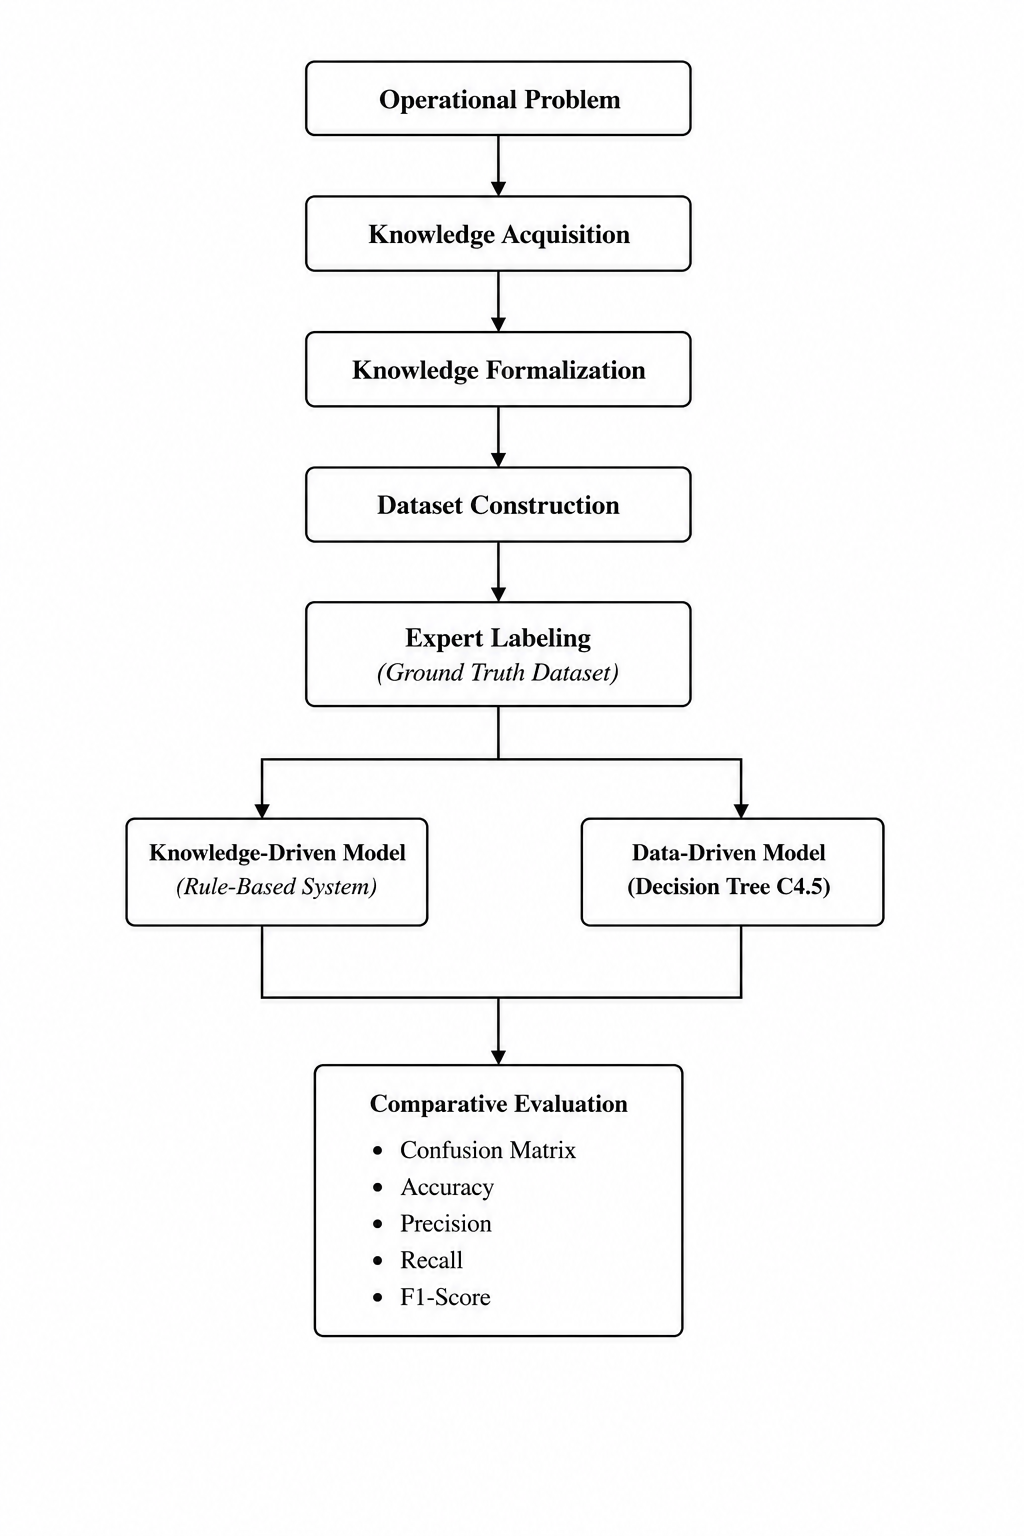
\includegraphics[width=0.82\columnwidth]{research_framework-1.png}
\caption{Proposed Research Framework}
\label{fig:research_framework}
\end{figure}

Tahapan pada kerangka penelitian tersebut dijelaskan secara rinci pada bagian \textit{Knowledge Acquisition}, \textit{Knowledge Formalization}, \textit{Dataset Construction}, \textit{Expert Labeling}, pembangunan model \textit{Rule-Based}, pembangunan model Decision Tree C4.5, serta evaluasi komparatif.

```latex
\subsection{Knowledge Acquisition}

Tahap \textit{Knowledge Acquisition} bertujuan untuk mengidentifikasi dan mengumpulkan pengetahuan operasional yang digunakan dalam proses penentuan prioritas pengiriman invoice. Pada penelitian ini, pengetahuan tidak hanya diperoleh dari data historis, tetapi juga dari aturan operasional pelanggan dan pengalaman staf administrasi. Seluruh informasi yang diperoleh pada tahap ini menjadi dasar dalam proses \textit{Knowledge Formalization} untuk membangun aturan keputusan dan atribut penelitian.

\subsubsection{Customer Regulation}

Regulasi pelanggan merupakan sumber pengetahuan eksplisit yang menjelaskan aturan administrasi setiap pelanggan. Informasi yang dikumpulkan meliputi jenis \textit{cut-off}, nilai \textit{cut-off}, jadwal penerimaan invoice, serta hari operasional penerimaan dokumen. Aturan tersebut digunakan untuk memahami karakteristik operasional masing-masing pelanggan dan menjadi acuan dalam proses penentuan prioritas pengiriman.

\subsubsection{Historical Invoice Data}

Data historis invoice digunakan untuk menggambarkan aktivitas operasional perusahaan yang sebenarnya. Dataset ini memuat informasi seperti nomor invoice, pelanggan, tanggal penerimaan invoice, tanggal pengiriman, dan riwayat distribusi. Data historis digunakan untuk mengidentifikasi pola pengiriman invoice sekaligus menjadi dasar dalam proses pembangunan dataset penelitian.

```latex
\subsubsection{Expert Knowledge}

Selain data operasional, penelitian ini juga memanfaatkan pengetahuan dari staf administrasi yang berpengalaman dalam menentukan prioritas pengiriman invoice. Pengetahuan tersebut digunakan untuk mengidentifikasi pertimbangan operasional yang belum terdokumentasi serta menyusun pedoman \textit{expert labeling}.

Hasil dari tahap \textit{Knowledge Acquisition} adalah kumpulan pengetahuan operasional yang diperoleh dari regulasi pelanggan, data historis invoice, dan pengetahuan pakar. Ringkasan sumber pengetahuan, informasi yang dikumpulkan, dan tujuan penggunaannya disajikan pada Tabel~\ref{tab:knowledge_acquisition}. Selanjutnya, pengetahuan tersebut digunakan sebagai masukan pada tahap \textit{Knowledge Formalization} untuk membentuk atribut penelitian dan aturan keputusan yang digunakan dalam proses pemodelan.

\begin{table}[htbp]
\caption{Knowledge Sources in the Knowledge Acquisition Stage}
\label{tab:knowledge_acquisition}
\centering
\renewcommand{\arraystretch}{1.2}
\resizebox{\columnwidth}{!}{
\begin{tabular}{|p{0.22\columnwidth}|p{0.32\columnwidth}|p{0.32\columnwidth}|}
\hline
\textbf{Knowledge Source} &
\textbf{Collected Information} &
\textbf{Purpose} \\
\hline

Customer Regulation &
Cut-off policy, cut-off value, receiving schedule, receiving day &
Capture explicit operational rules for each customer. \\
\hline

Historical Invoice Data &
Invoice number, customer, receive date, delivery date, delivery history &
Represent historical operational activities and support dataset construction. \\
\hline

Expert Knowledge &
Priority criteria, operational considerations, delivery decision strategy &
Develop labeling guidelines and validate operational rules. \\
\hline

\end{tabular}
}
\end{table}
```

\input{sections-indonesia/04_results}
\input{sections-indonesia/05_conclusion}

% --- PEMANGGILAN BIBTEX ---
\bibliographystyle{IEEEtran}
\bibliography{references}

\end{document}
